\chapter{Stand der Forschung}
Für die Untersuchung des Phasendiagramms eines 2DES auf dünnen Heliumfilmen ist die  verlässliche Erzeugung von hohen Elektronendichten eine unbedingte Voraussetzung. Nachdem das System Elektronen auf Bulk"=Helium nach seiner Entdeckung sehr umfassend  erforscht wurde, gab es erst über zehn Jahre später fundierte Erkenntnisse über den Grenzbereich eines 2DES auf dünnen Heliumfilmen. Eine Ursache für diese lange Zeitspanne ist sicherlich die große Herausforderung der reproduzierbaren Präparation des 2DES auf dünnen Heliumfilmen. Im Gegensatz zu Bulk"=Helium spielt hier der Einfluss des darunter liegenden Substrats eine große Rolle und erschwert es, von Messung zu Messung vergleichbare Ausgangsbedingungen sicherzustellen. 
  
\section{Elektronensysteme hoher Dichten}
\name{Etz} \ea\ \cite{Etz84} erreichten auf einem unbehandelten Silizium"=Substrat, also einer nur mit der natürlich vorhandenen Oxidschicht bedeckten Oberfläche, im Nichtgleichgewicht Elektronendichten bis zu \unit[$7\times10^{14}$]{\Em}. Allerdings konnte diese hohe Elektronendichte nur bei kontinuierlicher Nachlieferung von Elektronen gehalten werden und relaxierte nach Abschalten der Elektronenquelle innerhalb von Minuten auf deutlich geringere Werte unter \unit[$5\times10^{13}$]{\Em} zurück. Im Laufe dieser Experimente wurde die Abhängigkeit der Dicke des Heliumfilms von der Elektronendichte im 2DES \eqref{eqn:beladene_filmdicke} mit Hilfe der optischen Methode der Ellipsometrie am Heliumfilm bestimmt. Damit wurde eine Möglichkeit zur Verfügung gestellt, die Elektronendichte auf dünnen Heliumfilmen unabhängig von der an das Substrat angelegten Haltespannung zu bestimmen und somit den daraus bestimmten Dichtewert zu verifizieren.

Eine erste Messung des Phasenübergangs von der Elektronenflüssigkeit in das Wigner"=Regime auf einem gesättigten Heliumfilm wurde von \name{Jiang} \ea\ \cite{Jia88} gezeigt. Hierbei wurde auf einem Glassubstrat eine maximale Elektronendichte von \unit[$1.3\times10^{14}$]{\Em} erreicht. Die von den theoretischen Arbeiten von \name{Peeters} \ea{} \cite{Pee83, Pee84} vorhergesagte Modifikation des Phasendiagramms von 2DES auf dünnen Heliumfilmen konnte qualitativ verifiziert werden. Eine Korrektur des theoretischen Modells an die gemessenen Daten wurde von \name{Saitoh} \cite{Sai89} für eine quantitative Interpretation der Daten von \name{Jiang} \ea\ gegeben.

Um die Probleme der Detektion des Beweglichkeitssignals eines 2DES auf dünnen Heliumfilmen zu verringern, wurde versucht, die Messfrequenz, die bei den bekannten Messungen mit Sommer"=Tanner"= oder Corbino"=Geometrie in der Größenordnung von \unit[100]{kHz} liegt, weiter zu erhöhen. Eine Erhöhung der Messfrequenz bei vergleichbarer Amplitude des elektrischen Feldes hat eine Reduzierung der Schwingungsamplitude der Elektronen zur Folge. Bei geringerer Schwingungsamplitude erhoffte man sich eine schwächere Abhängigkeit der gemessenen Signale von den Einflüssen der vorhandenen Substratrauigkeit -- dies war der Beginn einer Reihe von Mikrowellenmessungen.

\section{Bisherige Mikrowellenmessmethoden}
\subsection{Messung der Transmission bei konstanter Anregungsfrequenz}
Von \name{Lehndorff} \cite{lehndorff} wurden die ersten Messungen an einem 2DES auf dünnen Heliumfilmen im Inneren eines Mikrowellen"=\HR s durchgeführt. Von Beginn an wurde wegen seiner geringen Leitfähigkeit bei tiefen Temperaturen Silizium als Substratmaterial verwendet. Für das Isolatormaterial zwischen dem Silizium und dem das 2DES tragenden Heliumfilm wurden isolierende Folienmaterialien, wie z.\ B. Hostaphan eingesetzt.

Zu Beginn der Mikrowellenmessungen war die naheliegende Messmethode, die Mikrowellen mit konstanter Frequenz in das System einzustrahlen, um somit z.~B. mit Hilfe einer an der Flanke der Mikrowellenresonanz liegenden Messfrequenz die Änderung der Resonanzfrequenz oder der Amplitude der Resonanz zu detektieren. Dies hat allerdings den Nachteil, dass es hierbei nicht möglich ist beide Größen voneinander zu trennen, da hierzu nicht genügend Messparameter zur Verfügung stehen.

\subsection{Regelung der Anregungsfrequenz auf die Position der Resonanzkurve}
Einen Fortschritt in der Messgenauigkeit und in der Trennung von Frequenz- und Amplitudenmessung brachte die Verwendung des in \cite{neser,guenzler} beschriebenen Lock"=In"=Regelkreises, mit dessen Hilfe die Messfrequenz immer mit der Resonanzfrequenz des \HR s mitgeführt wird. Diese Messmethode wird in Abschnitt~\ref{ssec:old_method} genauer beschrieben. 

Der Lock"=In"=Regelkreis hat den Nachteil, dass eine Änderung der Form der Resonanzlinie außerhalb der angenommenen mathematischen Beziehung von Güte und Transmission nicht zweifelsfrei detektiert werden kann, z.~B. bei einer Verkippung der Resonanzfrequenz und Modifikation der Linienbreite infolge von Leitungsreflexionen\footnote{In diesem Fall wird die frequenzabhängige Amplitude der gemessene Transmission durch einer Sinusoszillation mit einer Periode in der Größenordnung von \unit[10]{MHz} moduliert.}. Außerdem ergibt sich, wie in Abbildung~\ref{fig:absorption} im Abschnitt~\ref{sec:transquality} zu sehen ist, bei hoher Absorption des Elektronensystems eine Abweichung von der vorausgesetzten Abhängigkeit der Güte von der gemessenen Transmission. 

Ein Vorteil dieses Aufbaus ist allerdings, dass man schnelle Änderungen der Eigenschaften des Hohlraumresonators detektieren kann. Die Regelschleife wird mit der Messfrequenz des Lock"=In"=Verstärkers von einigen $\unit{kHz}$ betrieben, deshalb kann man hiermit auch noch Änderungen der Mikrowellen"=Resonanzkurve detektieren, die in der Größenordnung von Millisekunden liegen (wie z.B. der Einfluss des Filamentpulses auf die Resonanz oder die Auswirkungen der Bewegung der Oberfläche des flüssigen Heliums im Resonator).

\section{Vergleich einiger bisher durchgeführter Messungen}

\begin{table}[h!tp]
\begin{minipage}{0.98\textwidth}
\small
\begin{center}
\begin{tabular}{|r|c|c|c|c|c|}\hline
				& \cite{neser}& \cite{guenzler}\footnote{mit Korrektur nach \cite{bitnar}} & \cite{Gue96} & \cite{Mis97} & diese Arbeit\\\hline\hline
PMMA							& (PFPE)	& & & & \\\hline
Schichtdicke	 [nm]		& 5000	& & & & 100	\\
DK $\varepsilon_r$	& 1.7	&	&	& 2.2	& 1.7	\\
$T$ [K]				& 1.27	& & & & 1.29 \\
$d_0$ [nm]	& 30	& & & & 32 \\\hline
$n_\text{crit., WC}$ [$10^{14}]{\Em}$]	
										&	$\approx$120&	&	& 0.35	& 0.4 \\
$\Gamma_{WC}$	&	&	&	&	& 117 / 125	\\\hline\hline
\SiO								&	&	&	&	&	\\\hline
Schichtdicke	 [nm]		&	200 & 260	& 500	&	& 200	\\
DK $\varepsilon_r$	&	& 5 & 4 & & 4.5	\\
$T$ [K]				&	1.27 & 1.3 & & & 1.2	\\
$d_0$ [nm]	&	40 & 40 & & & 33		\\\hline
$n_\text{crit., WC}$ [$\unit[10^{14}]{\Em}$]
										&	2 & 4	& 1.3	&	& 2.0		\\
$\Gamma_{WC}$	&	& 160& & & 181/240	\\\hline
$n_\text{crit., QM}$ [$\unit[10^{14}]{\Em}$]
										&	& 33	& 4	& & 24	\\
$\Gamma_{QM}$	&	&	&	&	&	100/125	\\\hline
\end{tabular}
\end{center}
\end{minipage}
\caption{Vergleich verschiedener Resultate für 2DES auf dünnen Heliumfilmen.}
\label{tab:compare}
\end{table}

In Tabelle~\ref{tab:compare} sind charakteristische experimentelle Ergebnisse aus verschiedenen Veröffentlichungen von Messungen an 2DES auf dünnen Heliumfilmen aufgeführt. Deutlich wird hier eine starke Streuung der erhaltenen Gamma"=Werte für den Wigner"=Übergang. Auch bei den Veröffentlichungen \cite{guenzler,Gue96} zum sog.\ Quantenschmelzen, also dem Übergang vom Wigner"=Regime in das entartete Fermigas, finden sich stark abweichende Ergebnisse. Ein immer vorhandener Unsicherheitsfaktor ist die Bestimmung der aktuellen Elektronendichte aus der Haltespannung. Zum einen ist es für die Gültigkeit der erhaltenen Dichtewerte wichtig, dass sich das 2DES in Sättigung befindet (d.~h.\ $\vec E=0$ oberhalb des 2DES) und weiterhin spielen auch durchgebrochene Oberflächenladungen eine Rolle, da sie die scheinbare Sättigungsdichte zu höheren Elektronendichten verschieben.

\begin{figure}[h!tp]
	\begin{center}
	\subfigure[\cite{guenzler} mit Korrektur nach \cite{bitnar}]{%
		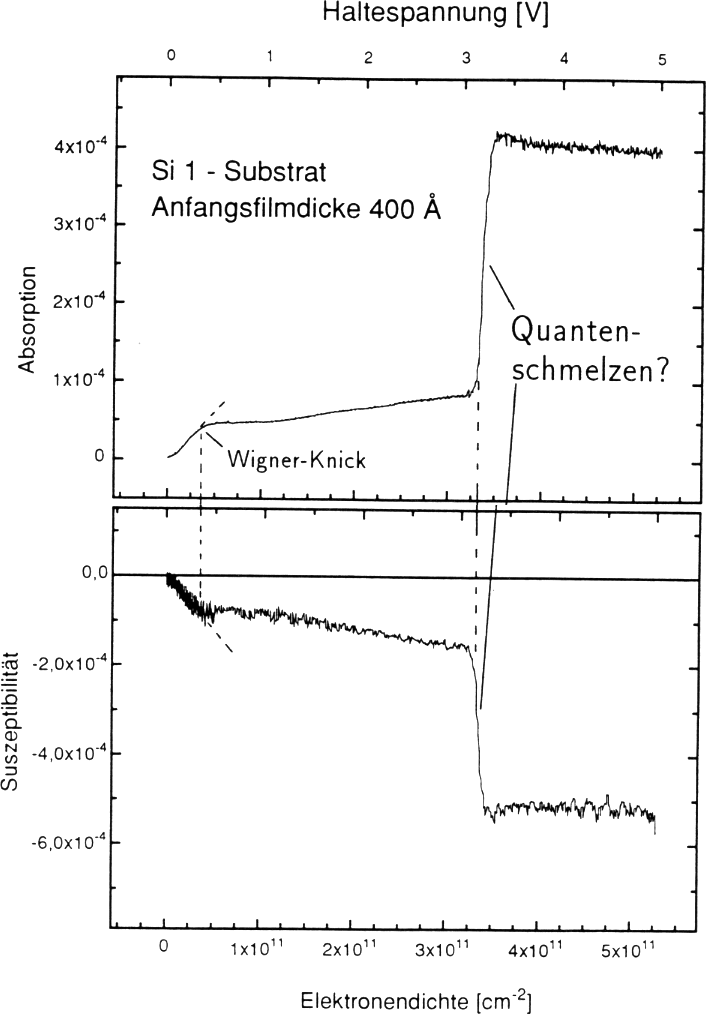
\includegraphics[width=\ssmallwidth]{stand_der_forschung/Bit95}}%
	\hspace{1cm}%
	\subfigure[\cite{Gue96}]{%
		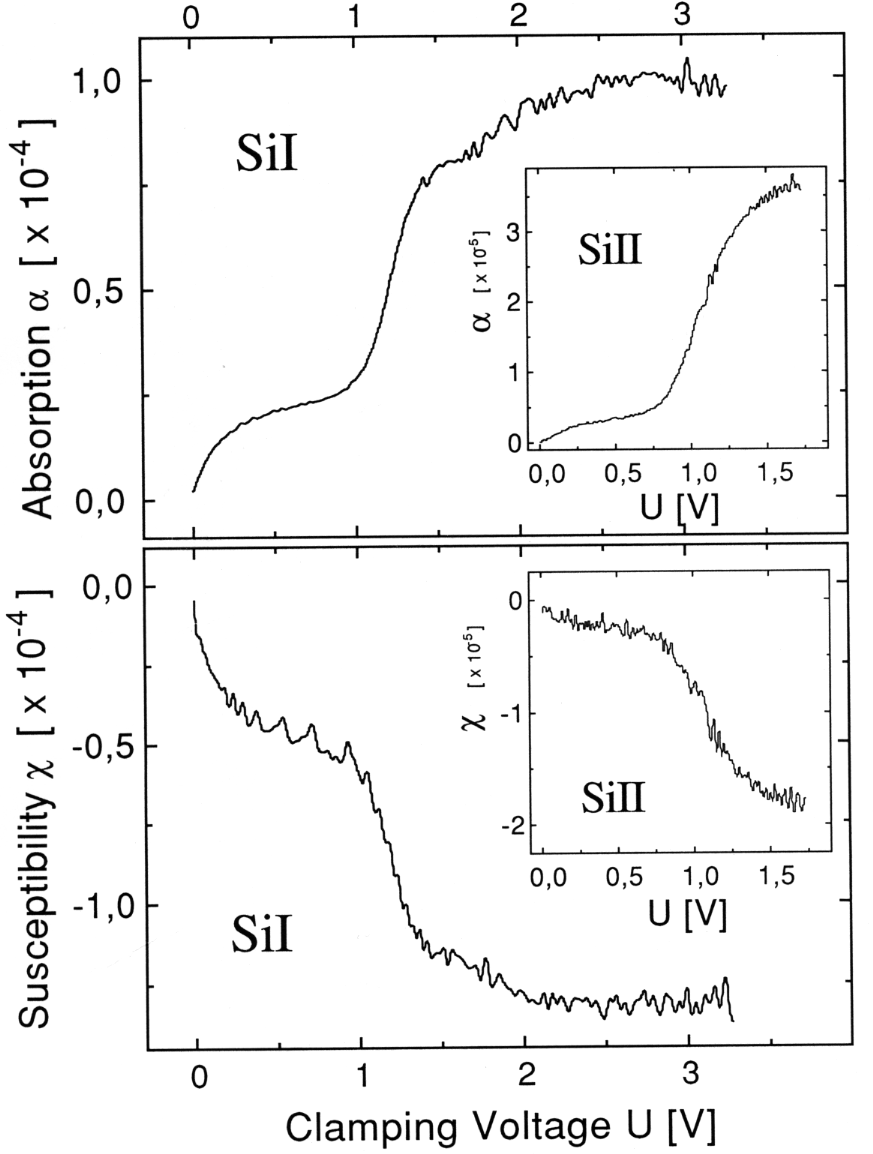
\includegraphics[width=\ssmallwidth]{stand_der_forschung/Gue96}}%
	\end{center}
	\caption{Bisher veröffentlichte Messungen des sog.\ Quantenschmelzens.}
	\label{fig:oldQM}
\end{figure}
In Abbildung~\ref{fig:oldQM} sind beide bisher veröffentlichte Messungen des sog.\ Quantenschmelzens gezeigt. In der Doktorarbeit von \name{T. Günzler} \cite{guenzler} wurden erstmals Anzeichen für einen Phasenübergang vom Wigner"=Festkörper zum entarteten Fermigas entdeckt. Allerdings wurden die hierbei erreichten Elektronendichten offensichtlich wegen der Annahme einer zu geringen Dicke der \SiO"=Deckschicht der Substrate um ca.\ einen Faktor 2.5 überschätzt. Die Filmdicke der Deckschicht wurde in der Diplomarbeit von \name{Bitnar} \cite{bitnar} jedoch nachgemessen und die bisher erhaltenen Elektronendichten korrigiert. Die darauffolgende Veröffentlichung von \name{Günzler} \ea\ \cite{Gue96} zeigt einen weiteren experimentellen Hinweis auf einen derartigen Phasenübergang.
 
Wenn man die experimentellen Ergebnisse zu den Phasenübergängen in das Fermi"=Regime in Tabelle~\ref{tab:compare} und Abbildung~\ref{fig:oldQM} {\bfseries (a)} und {\bfseries (b)} vergleicht, sieht man z.\ B. deutliche Unterschiede im Verhältnis der gemessenen kritischen Dichten $n_\text{crit., QM}$ und $n_\text{crit., WC}$. Dieses liegt bei \cite{guenzler} und dem in dieser Arbeit gezeigten Ergebnis bei ungefähr 10, während es bei \cite{Gue96} nur ca.\ 3 ist. 
 
\enlargethispage{\baselineskip}
Da der in Abbildung~\ref{fig:oldQM} {\bfseries (b)} gezeigte Wigner"=Knick vor allem bei der Probe SiII sehr ausgeschmiert ist, liegt die Vermutung nahe, dass dieser Teil der Messkurve als Artefakt ähnlich dem bei der zweiten Kurve in Abbildung~\ref{fig:pmma_reproduce} {\bfseries (a)} sichtbaren scheinbar früheren Beginn der Beladung interpretiert werden kann. Dieses Verhalten wurde bei der experimentellen Aufnahme von Serien von Beladekurven häufig beobachtet. Nach dem Durchlaufen einiger Beladezyklen scheint die Beladung mit Elektronen schon bei geringeren Haltespannungen einzusetzen. Zusätzlich erhält man beim Übergang in das übliche Drude"=Verhalten einen zweiten Knick im Verlauf der Transmission.

In der Abbildung~\ref{fig:qm_wigner} wurden die aus der Abbildung~\ref{fig:oldQM} {\bfseries (b)} digitalisierten Daten unter der Annahme ausgewertet, dass der in den Absorptionsdaten deutlich sichtbare Phasenübergang nicht ins Quanten"=Regime führt, sondern den bekannten Übergang zum Wigner"=Festkörper darstellt.
\begin{figure}[h!tbp]
	\centerline{
	\subfigure[digitalisierte Daten nach \cite{Gue96}]{\plotlink{Gue96_test}{\includegraphics[width=\smallwidth]{stand_der_forschung/Gue96_test}}}\hfill%
	\subfigure[Auswertung des \name{Wigner}"=Übergangs: {$n_\text{crit}=\unit[1.4\times10^{14}]{\Em}$},  $\Gamma=214$]{\plotlink{Gue96_test2}{\includegraphics[width=\smallwidth]{stand_der_forschung/Gue96_test2}}}}
	\caption[Alternative Interpretation der Daten aus \cite{Gue96}]{Andere Möglichkeit der Interpretation der Messdaten von \cite{Gue96}. Könnte es sich hierbei um einen \name{Wigner}"=Übergang handeln? (siehe Text)}
	\label{fig:qm_wigner}
\end{figure}
\enlargethispage{2\baselineskip}
Die erhaltenen Daten $n_\text{crit}=\unit[1.4\times10^{14}]{\Em}$ und $\Gamma=214$ liegen durchaus im erwarteten Bereich.
Leider waren die Originaldaten der Messung nicht verfügbar, die zur Überprüfung dieser Vermutung einen tieferen Einblick in den gesamten Ablauf und der Vorgeschichte des dargestellten Ausschnitts der Messung ermöglichen würden.
 

